\section{Parte 3}

El proceso de Sharding consiste en guardar una base de datos a través de muchas máquinas. Esta es la forma en la que MongoDB provee una alternativa para soportar escalabilidad en casos donde la cantidad de datos o el volúmen de pedidos sobre la base excede a las capacidades de una única máquina, mecanismo conocido como "horizontal scaling".

En particular, MongoDB provee dos estrategias de sharding que difieren en su forma de distribuir los registros de datos a través de las distintas máquinas disponibles en función del valor de un atributo dado de los documentos, definido como la clave.

\begin{itemize}
  \item Sharding por range: los datos comienzan almacenados en una única máquina, y a medida que crece el volúmen de datos se mantiene una estadística del rango donde están contenidos todos los valores del atributo clave de los registros que fueron insertados. Cuando el tamaño del primer shard supera un determinado umbral, se realiza una partición en el espacio de las claves y se distribuyen equitativamente los registros.
  \item Sharding por hashing: ante la inserción de un nuevo documento, se aplica una función hash sobre el atributo clave, luego determinando a partir del resultado cuál será el número de shard correspondiente para el nuevo registro. Se busca generalmente que la función de hash distribuya los datos uniformemente, de forma tal que un nuevo documento tenga una probabilidad de aproximadamente $\frac{1}{\#shards}$ de ser asignado a cada shard.
\end{itemize}

En general, cualquier base de datos de gran volúmen y/o pedidos que cuente con un atributo propicio para actuar de clave es un potencial caso de uso para sharding. Si adicionalmente los registros poseen una partición natural que podría beneficiarse al ser alojados en distintas máquinas, los incentivos son aún mayores. Un ejemplo de esto podría ser una base de datos de usuarios divididos por regiones (ej, clientes de latinoamérica, clientes de Europa, clientes de Asia). Otros casos típicos son bases de datos de entidades numeradas o con identificadores numéricos como libros identificados por su ISBN, o vehículos distribuídos según su TAN.

\subsection{Experimentación y consideraciones}

Configuramos una instalación de MongoDB en modo Sharding, con un total de 5 shards locales (es decir, 5 procesos ejecutándose en una misma máquina, pero funcionando autónomamente como si se encontraran en distintos dispositivos). En el caso de ambas estrategias de sharding, realizamos un experimento consistente en insertar 500.000 documentos en una colección en modo sharding, midiendo cada 20.000 inserciones el estado actual de los shards activos.

En una primera instancia, repetimos el experimento diez veces con sharding en modo range, y en segundo lugar, lo repetimos diez veces en modo hashed. El estado observado luego de cada iteración de 20.000 inserciones fue la cantidad total de documentos almacenados en cada shard.

Como clave para el proceso de sharding, fue elegido un id entero arbitrario tomado de forma aleatoria y sin repetición en el intervalo 0 ... 500.000. Esta elección respeta los lineamientos generales para obtener buena performance a partir de la elección de clave\footnote{https://docs.mongodb.com/manual/tutorial/choose-a-shard-key/}: el espacio de claves es divisible efectivamente (entre dos claves cualquieras, es sencillo definir el rango de claves que están en medio de ellas), y adicionalmente las claves tienen una distribución uniforme dentro del espacio permitido (ninguna parte del espacio de claves es más densa que otra).

\subsection{Resultados}

En primer lugar, mostramos la progresión en los tamaños de los distintos shards en función de la cantidad de iteraciones. Esto permite analizar la distribución de datos entre los distintos shards, y hasta qué punto la misma es uniforme. Esto se puede observar en las figuras \ref{fig:publicaciones-ranges} y \ref{fig:publicaciones-hashed}.

\begin{figure}[h!]
  \centering
  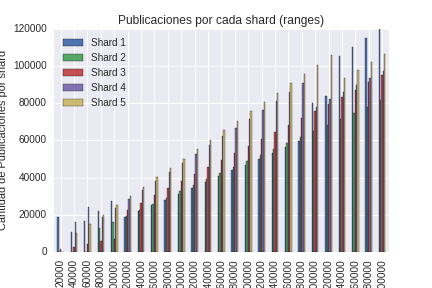
\includegraphics[width=4in]{imagenes/publicaciones_by_shard_ranges.png}
  \caption{Cantidad de documentos por shard (ranges).}
  \label{fig:publicaciones-ranges}
\end{figure}

\begin{figure}[h!]
  \centering
  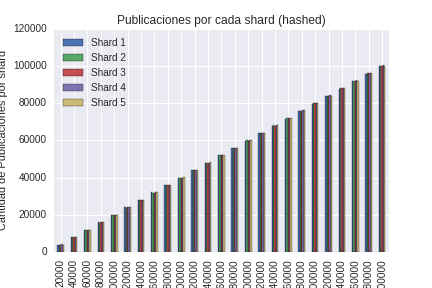
\includegraphics[width=4in]{imagenes/publicaciones_by_shard_hashed.png}
  \caption{Cantidad de documentos por shard (hashed).}
  \label{fig:publicaciones-hashed}
\end{figure}

Al inspeccionar las figuras, se observa cómo efectivamente los datos se distribuyen entre los distintos shards, dado que la cantidad de documentos almacenados en cada shard crece linealmente con el tamaño total de la colección.

Notablemente, la distribución en el caso de sharding por hashing es prácticamente ideal. La función de hash aplicada sobre todos los elementos de un conjunto aleatorio uniforme presenta en mayor medida una distribución aleatoria uniforme.

El comportamiento en el caso de sharding por rangos no muestra la misma uniformidad. Luego de la primera tanda de inserciones, casi el 100\% de los documentos se encuentran almacenados en el primer shard. A partir de la segunda tanda, se comienzan a utilizar todos los shards pero con una distribución fuertemente sesgada hacia los shards 1 y 4. A medida que la cantidad de documentos es mayor, la distribución muestra una estructura más regular y más homogénea, aunque siempre con un fuerte sesgo hacia el shard 1.

El hecho de que el comportamiento de la distribución con sharding por rangos sea más errático durante las primeras tandas de inserciones, se explica con el hecho de que, al comenzar el experimento, MongoDB no tiene información alguna sobre la distribución o los rangos de las claves de los documentos que se ingresarán a la base. A medida que se realizan más inserciones, la estimación en tiempo real de MongoDB es cada vez más precisa respecto al rango verdadero del set de claves, permitiendo una mejor distribución de los documentos entre los distintos shards.
